\documentclass{article}
\usepackage[utf8]{inputenc}
\usepackage{graphicx}
\title{Assignment 4 Project Management Agile Development}
\author{Himanshu Patel (C0735691), Shubham (C0737342), Sujalkumar Patel (C0735603)\\Jattinder Kaur (C0737459), Palwinder Kaur (C0737690), Navneet Kaur (C07354154)}

\date{August 2019}

\begin{document}

\maketitle

\section{Team Members}
Himanshu Patel (C0735691), Shubham (C0737342), Sujalkumar Patel (C0735603)\\Jattinder Kaur (C0737459), Palwinder Kaur (C0737690), Navneet Kaur (C07354154)

\includegraphics[width=8cm]{panda.png}

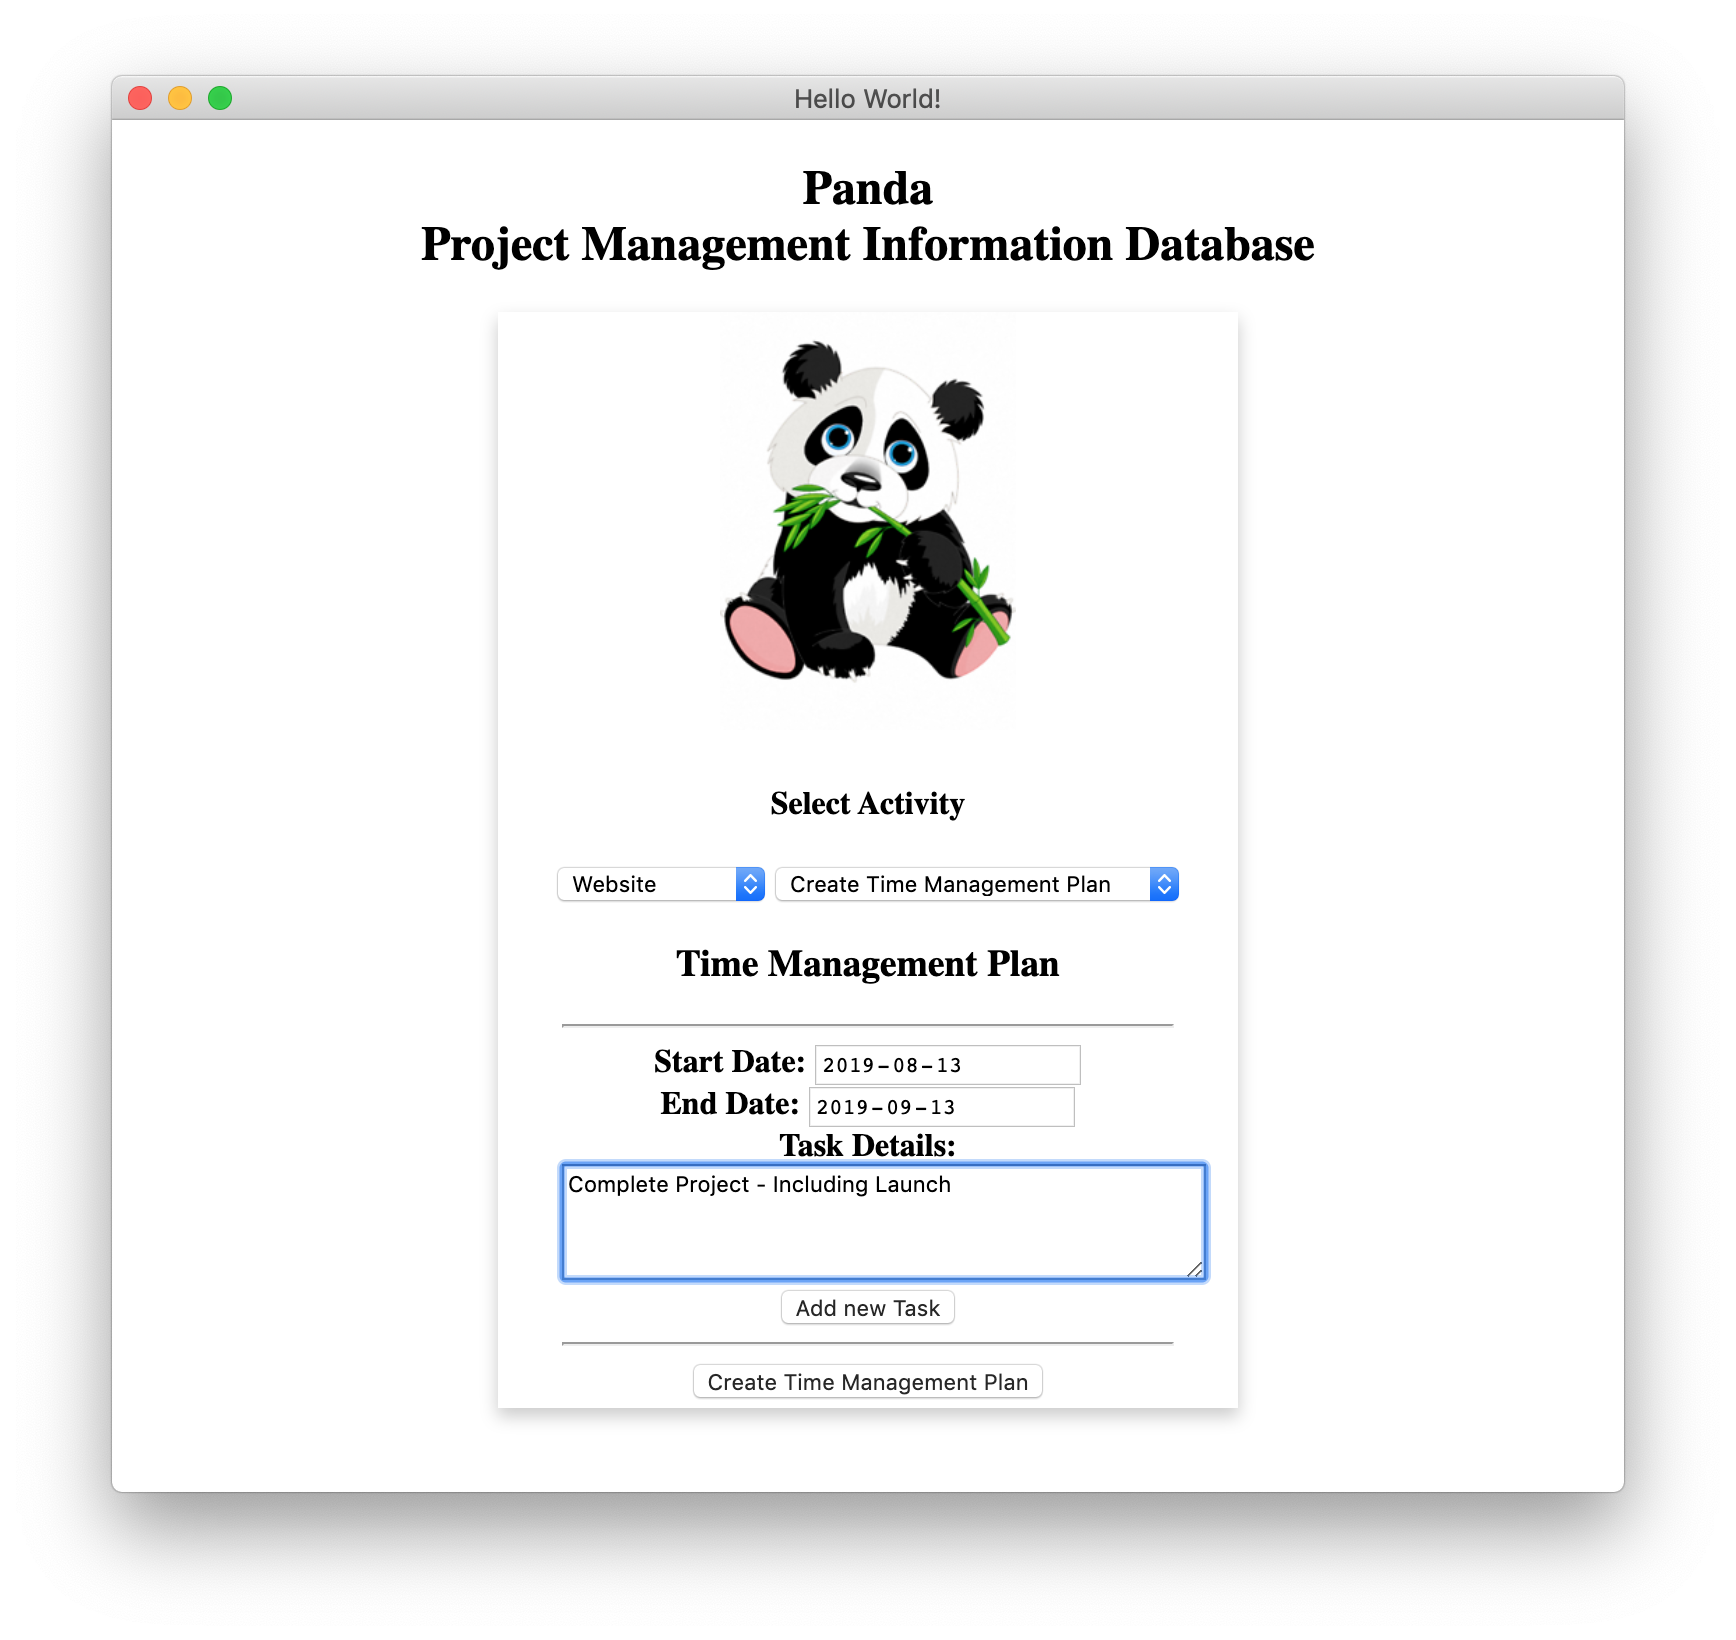
\includegraphics[width=16cm]{screenshot.png}

\newpage
\section {Our Web Application Code:}
\begin{verbatim}
<!DOCTYPE html>
<html>
<head>
<meta name="viewport" content="width=device-width, initial-scale=1">
<style>

html {
  text-align: center;
}

.card {
  box-shadow: 0 4px 8px 0 rgba(0,0,0,0.2);
  transition: 0.3s;
  margin: auto;
  width: 50%;
  
}

.card:hover {
  box-shadow: 0 8px 16px 0 rgba(0,0,0,0.2);
}

.container {
  padding: 2px 16px;
  text-align:center
}



</style>
</head>
<body>

<h2>Panda<br>Project Management Information Database</h2>

<div class="card">
  
  <img src="panda.png" alt="Avatar" style="width:40%">
  <div class="container">
    <h4><b>Select Activity</b></h4> 

    <select name="cars">
        <option value="Select Project">Select Project</option>
        <option value="saab">Website</option>
        <option value="fiat">Mobile App</option>
        
      </select>

    <select name="cars">
        <option value="Select Activity">Select Activity</option>
        <option value="saab">Create Time Management Plan</option>
        <option value="fiat">Create Cost Management Plan</option>
        <option value="audi">Create Quality Management Plan</option>
      </select>

      <form action="/action_page.php">
        <div class="container">
          <h3>Time Management Plan</h3>
          <hr>
      
          <label for="email"><b>Start Date: </b></label>
          <input type="date" placeholder="Enter Start Date" name="email" required>
          <br>
          <label for="psw"><b>End Date: </b></label>
          <input type="date" placeholder="Enter End Date" name="psw" required>
          <br>
          <label for="psw-repeat"><b>Task Details: </b></label>
          <textarea rows="4" cols="50" name="comment" form="usrform">
              Enter details here...</textarea>

              <button type="submit" class="registerbtn">Add new Task</button>
          <hr>
          
          <button type="submit" class="registerbtn">Create Time Management Plan</button>
          
        </div>
       
      </form>

  </div>
</div>

</body>
</html> 
\end{verbatim}

\section {Why we choose to implement our UML Objects in this way in our Web App (Our HTML PAGE)}

Assignment 3 file is been uploaded to GitHub for refrence\\

We Choose to provide Project manager with the list of projects in Dropdown list so he can select project and choose activities to perform such as Create Time Management Plan, Create Cost Management Plan, Create Quality Management Plan.

Based on which Manager fill the form to create Plans for Project.


\section{Github URL}
https://github.com/imhsp/Electron

\end{document}
